% !TEX root = ../thesis_main.tex

\section{BSA as a prolate ellipsoid}
\graphicspath{{rom_studies/figs/}}

The crystal structure of the BSA (pdb 4f5s) used in our simulations corresponds
to a dimer. Knowing that this structure can be modeled as an ellipsoid \cite{SquireETal1968},
we look for different alternatives to decide the dimensions of the ellipsoid. We took two
different approaches, a surface model and a volume model. The first attempt is 
the surface model which consists on finding the dimensions
of an ellipsoid that encapsules all the charges within the protein. We determined the principal axes of this
ellipsoid using Principal Component Analysis. Principal component analysis is a technique that
uses orthogonal transformations and brings out patterns in a set of data. When 
we use a PCA in three dimensions, these transformations ensure that the first 
component is the one with most variation, the second one is the second-most, and
third one the least. This technique provided us the three eigenvectors that best 
describe the cloud of mesh-vertices. The values of the principal axis are $a=98.9\, \text{\AA}$, $b=54.2\, \text{\AA}$, and $c=41.8\, \text{\AA}$. 
Using these vectors when creating the mesh of the ellipsoid ensures that all the charges are contained.
The second approach to model the BSA is to create an ellipsoid that matches the volume of the BSA. To find the dimensions 
of the volume-equivalent equivalent we made some approximations. We obtained the volume of the BSA protein original mesh
using Trimesh (\url{https://github.com/mikedh/trimesh})), and looking at the PCA principal axis we notice that $b$ and $c$ are close 
compared to $a$, then $b=c=x$ and $a$ is double the size $a=2x$, agreeing with the results from Squire and co-workers
\cite{SquireETal1968}. Using these approximations we can write the volume of the ellipsoid:

\begin{equation}
    V_e = \frac{4\pi}{3}a\,b\,c 
\end{equation}

as 

\begin{equation}
    V_e = \frac{4\pi}{3}2\,x^3
\end{equation}

Knowing that the volume of the volume of the BSA protein is $V_e = 166642 \, \text{\AA}^3$ we get that $x=27.09496 \, \text{\AA}$ 
and therefore $a=54.18993 \, \text{\AA}$ and $b=c=27.09496 \, \text{\AA}$. These dimensions give us an ellipsoid that hast the same volume 
as the original BSA mesh, however, we can not encapsule all the charges inside of it. To be able to use this model we needed to study first the 
effects of replacing the distribution of charges by a monopole, as well as the possibility of not include them in the model. 

\subsection{Effect of charges within the protein}

Since the PCA model can encapsuled all the charges we intended to use this model to study the effect of using the charges distribution, versus
a monopole representation of the charges ("center of mass"), and also no charges present. To ensure that we are solving the equations properly, 
we perform a convergence analysis.


\subsubsection{PCA ellipsoid convergence analysis}

We performed a grid convergence analysis on the PCA (Principal component analysis) ellipsoid - sensor system containing a full pqr (see Figure \ref{fig:one_pca_sketch}). 
Since we compute the extinction cross section of the sensor (8 nm radius silver sphere), we set a fixed mesh density for the ellipsoid and refine 
the mesh of the sphere ($N=512, 2048, 8192, 32768$). We found that a mesh with $N=5120$ elements for the ellipsoid was fine enough for the convergence analysis.
We used the same physical conditions and parameters that were used for the BSA-nanoparticle convergence analysis presented in
\ref{sec:grid_conv_bsa}. Similarly to the BSA-sensor system, the distance between the sensor and the PCA-ellipsoid 
was $d=1$ nm, and the ellipsoid was oriented such that the dipole moment of the charges was aligned with the $y$-axis. To obtain the error 
estimate we used Richardson extrapolated value of the extinction cross section as a reference, $C_{ext} = 1432.6560$ nm$^2$.
The observed order of convergence is $0.99$, and Figure \ref{fig:err_sph-pca} shows that the error decays with the number of boundary elements ($1/N$). This provides
evidence that the numerical solutions computed with \pygbe are correctly resolved by the meshes.  Table \ref{table:err_sph-pca} shows the percentages error for the different 
meshes used in this study.

\begin{figure}%[h] %  figure placement: here, top, bottom, or page
    \centering
    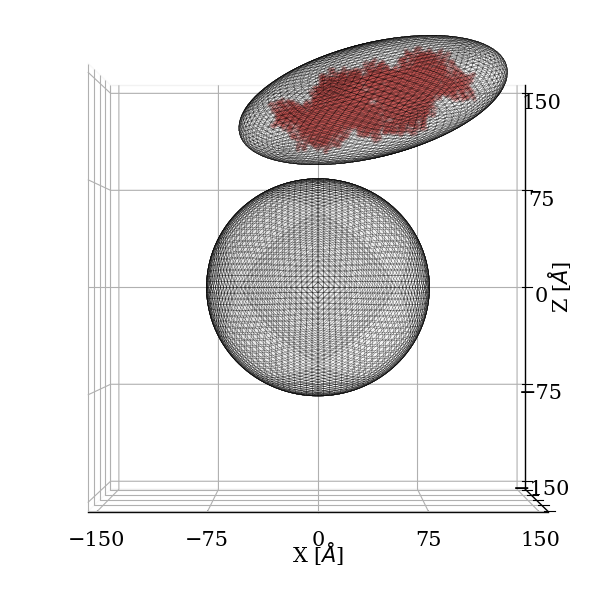
\includegraphics[width=0.65\textwidth]{viz/one_pca_full_display.png} 
    \caption{Sensor protein display: PCA ellipsoid with charges distribution located at $\pm 1$ nm of the 
    nanoparticle in the $z$-direction.}
    \label{fig:one_pca_sketch}
 \end{figure}


\begin{figure}%[h] %  figure placement: here, top, bottom, or page
    \centering
    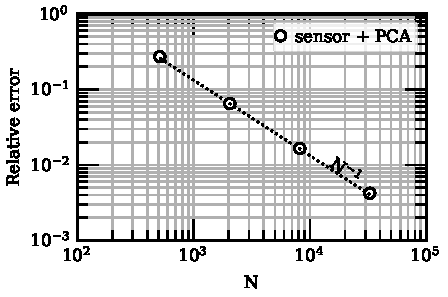
\includegraphics[width=0.85\textwidth]{convergence_sensor_pca_w380.pdf} 
    \caption{Grid-convergence study of extinction cross-section of a spherical silver
             nanoparticle with a PCA ellipsoid which contains 
             the charges distribution within it, located at $d=1$ nm.}
    \label{fig:err_sph-pca}
 \end{figure}

 \begin{table}%[h]
    \centering
    \caption{\label{table:err_sph-pca} Estimated percentage error of the PCA ellipsoid-sensor 
    system, with respect to the extrapolated value (using Richardson extrapolation).} 
    \begin{tabular}{c c}
    \hline%\toprule
    N & \% error \\
    \hline%\midrule
     $512$ & $27.2$ \\
     $2048$ & $6.5$ \\
     $8192$ & $1.66$ \\
     $32768$ & $0.42$ \\
    \hline%\bottomrule
    \end{tabular}
\end{table}

After performing the convergence analysis studies, we relaxed the numerical parameters of the computations to reduce the run-time without 
compromising accuracy. The following parameters were used to obtain all non-convergence results presented from now on for the case of PCA ellipsoids.

\begin{table}%[h]
    \centering
    \caption{\label{table:rel_pca_par} Relaxed parameters for the PCA ellipsoid case. The parameters that are not 
    mentioned here remain the same as in the convergence study.} 
    \begin{tabular}{c c}
    \hline%\toprule
    parameter & \% value \\
    \hline%\midrule
     $N_{sensor}$ & $8192$ \\
     $k_{fine}$ & $19$ \\
     $P$ & $6$ \\
     $tol$ & $1\times 10^{-3}$ \\
    \hline%\bottomrule
    \end{tabular}
\end{table}

The Richardson extrapolated value for the PCA case is: $1432.6561$ nm$^2$ and the computed value with the relaxed parameters 
is $1456.0781$ nm$^2$. If we compute the percentage error we obtain $1.63 \%$.

\subsubsection{Charges model analysis} \label{ssub:pqr_analysis}

In order to know if we could use a VE approach we studied the effect of the charges inside the protein. We analyzed
the different representations of pqr (full distribution and equivalent monopole) as well as the impact of having
no charges present. The setup of the simulations consists in a silver sphere sensor ($r=8$ nm) with a PCA ellipsoid 
at 1 nm of the surface of the sensor in the $z$-direction, oriented such that the dipole moment is aligned with the $y$-axis. We run 
three different cases, one with the full charges distribution, a second case with one equivalent charge located in the
"center of mass" (See Figure \ref{fig:one_pca_cm_sketch}), and lastly an empty ellipsoid with no charges. Figure 
\ref{fig:pqr_pca} shows the results for the different models of the charge distribution as well as the results when 
there are no charges present within the ellipsoid. 

\begin{figure}%[h] %  figure placement: here, top, bottom, or page
    \centering
    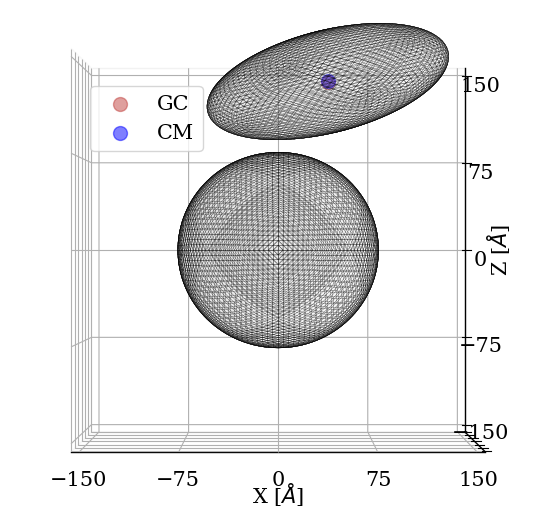
\includegraphics[width=0.65\textwidth]{viz/one_pca_cm_gc_display.png} 
    \caption{Sensor protein display: PCA ellipsoid with equivalent monopole charge, located at $\pm 1$ nm of the 
    nanoparticle in the $z$-direction. The label "CM" indicates center of mass where the monopole charge is located, and
    the label "GC" indicates the geometric center for reference.}
    \label{fig:one_pca_cm_sketch}
 \end{figure}



\begin{figure}%[h] %  figure placement: here, top, bottom, or page
    \centering
    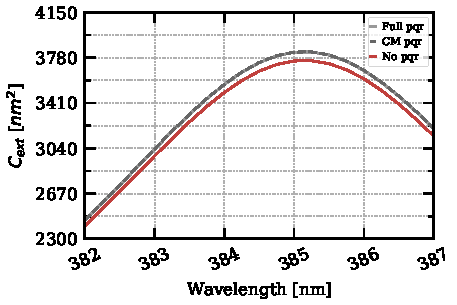
\includegraphics[width=0.85\textwidth]{pqr_analysis_pca.pdf} 
    \caption{Extinction cross-section as a function of wavelength for an $8$ nm
    silver sphere immersed in water with one PCA ellipsoid at $1$ nm away from 
    the surface in the $z$-direction, under a constant electric field on the $z$-direction.
    The label "Full pqr" corresponds to the full distribution of charges, the label "CM pqr" corresponds to a monopole representation 
    of the charges obtained by computing the center of mass of them, and the label "No pqr" 
    corresponds to the case where there are no charges present.}
    \label{fig:pqr_pca}
 \end{figure}

 The maximum value for all the curves in Figure \ref{fig:pqr_pca} occurs at $385.25$ nm. The 
 maximum value of the extinction cross section for the full distribution ("Full pqr") is $3827.06$ nm$^2$ and for 
 the monopole/center-of-mass representation ("CM pqr") is $3828.21$ nm$^2$, what results in a difference of $0.03 \,\%$. The
 maximum value of the extinction cross section when there are no charges present ("No pqr") is $3755.51$ nm$^2$ which compared to 
 the maximum for the full distribution gives us a difference of $1.87 \,\%$. Looking at these results we can say that the presence of 
 charges inside the protein does not affect the wavelength shift. However, it does affect the intensity of the maximum value of the 
 extinction cross section by approximately $2 \,\%$. Finally, we can say that using a monopole approximation for the distribution of charges, 
 is equivalent to using the full distribution of charges.

\subsection{Surface equivalent vs Volume equivalent} \label{ssec:surf_vol_ell}

In section \ref{ssub:pqr_analysis} we show that using a monopole approximation is equivalent to using the full distribution of charges. This 
allow us to explore the effects of the volume equivalent model. Similarly to the PCA case we need to perform convergence analysis for
the volume equivalent case, we present the results of the convergence analysis in section \ref{sssec:ve_conv}. Following the convergence 
study of the volume equivalent ellipsoid we present, in section \ref{sssec:ell_mod_comp}, the comparison of the PCA ellipsoid model and the volume equivalent 
model with the original BSA protein structure model, replicating the configuration shown in Figure \ref{fig:display_z}. 


\subsubsection{Volume Equivalent ellipsoid convergence analysis}\label{sssec:ve_conv}

We performed a grid convergence analysis on the VE (volume equivalent) ellipsoid - sensor system containing a monopole charge located 
in the center of mass of the charge distribution. (see Figure \ref{fig:one_ve_sketch}). Since we compute the extinction cross section of the sensor 
(8 nm radius silver sphere), we set a fixed mesh density for the ellipsoid and refine 
the mesh of the sphere ($N=512, 2048, 8192, 32768$). We found that a mesh with $N=1280$ elements for the ellipsoid was fine enough for the convergence analysis.
We used the same physical conditions and parameters that were used for the BSA-nanoparticle convergence analysis presented in
\ref{sec:grid_conv_bsa}. Similarly to the BSA-sensor system, the distance between the sensor and the VE-ellipsoid 
was $d=1$ nm, and the ellipsoid was oriented such that the dipole moment of the charges was aligned with the $y$-axis. To obtain the error 
estimate we used Richardson extrapolated value of the extinction cross section as a reference, $C_{ext} = 1683.8117$ nm$^2$.
The observed order of convergence is $0.99$, and Figure \ref{fig:err_sph-ve} shows that the error decays with the number of boundary elements ($1/N$). This provides
evidence that the numerical solutions computed with \pygbe are correctly resolved by the meshes.  Table \ref{table:err_sph-ve} shows the percentages error for the different 
meshes used in this study.

\begin{figure}%[h] %  figure placement: here, top, bottom, or page
    \centering
    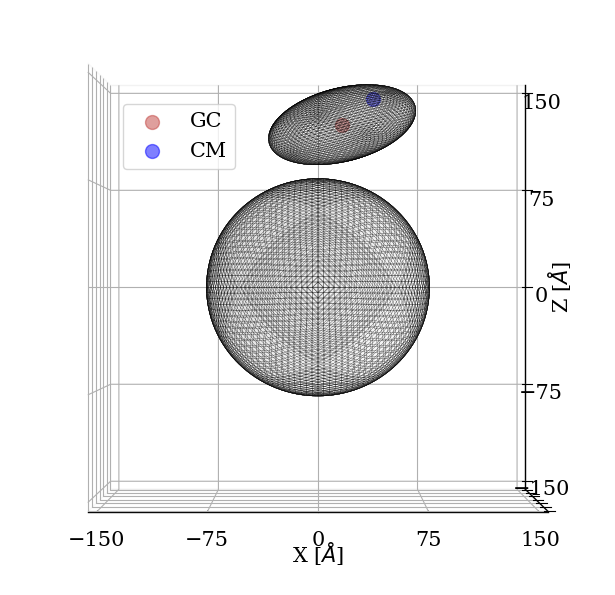
\includegraphics[width=0.65\textwidth]{viz/one_ve_cm_gc_display.png} 
    \caption{Sensor protein display: Volume equivalent ellipsoid with monopole charge ("CM"), located at $1$ nm of the 
    nanoparticle in the $z$-direction. The geometric center ("GC") is display for reference.}
    \label{fig:one_ve_sketch}
 \end{figure}


\begin{figure}%[h] %  figure placement: here, top, bottom, or page
    \centering
    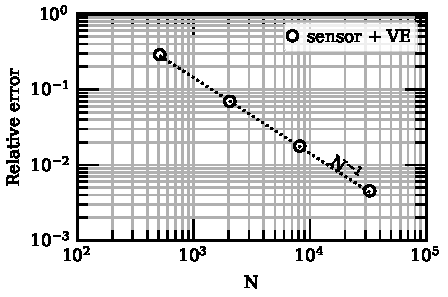
\includegraphics[width=0.85\textwidth]{convergence_sensor_ve_w380.pdf} 
    \caption{Grid-convergence study of extinction cross-section of a spherical silver
             nanoparticle with a volume equivalent ellipsoid at $d=1$ nm which contains 
             a monopole charge..}
    \label{fig:err_sph-ve}
 \end{figure}

 \begin{table}%[h]
    \centering
    \caption{\label{table:err_sph-ve} Estimated percentage error of the VE ellipsoid-sensor 
    system, with respect to the extrapolated value (using Richardson extrapolation).} 
    \begin{tabular}{c c}
    \hline%\toprule
    N & \% error \\
    \hline%\midrule
     $512$ & $28.8$ \\
     $2048$ & $6.96$ \\
     $8192$ & $1.78$ \\
     $32768$ & $0.45$ \\
    \hline%\bottomrule
    \end{tabular}
\end{table}

After performing the convergence analysis studies, we relaxed the numerical parameters of the computations to reduce the run-time without 
compromising accuracy. We use the parameters from Table \ref{table:rel_pca_par} to obtain all non-convergence results presented from 
now on for the case of VE ellipsoids. The Richardson extrapolated value for the VE case is: $1683.8117$ nm$^2$ and the computed value with 
the relaxed parameters is $1713.1972$ nm$^2$. If we compute the percentage error we obtain $1.75 \%$.

\subsubsection{Ellipsoid model vs original BSA}\label{sssec:ell_mod_comp}

In Figure \ref{fig:2pz_ell_resp} we show the results of comparing both ellipsoidal models of the protein with the 
original representation of the protein obtained from the crystal structure. We present the LSPR response 
of the system showed in Figure \ref{fig:display_z}, and for the ellipsoidal models we use an equivalent 
setup that replaces the proteins, located at $\pm 1$ nm in the $z$-direction, for the respective ellipsoids.
Both the PCA and VE model contain a monopole charge in the center of mass of the distribution.

\begin{figure} %[h] %  figure placement: here, top, bottom, or page
    \centering
    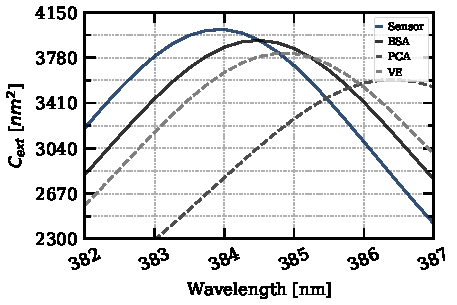
\includegraphics[width=0.85\textwidth]{two_ell_analysis.pdf} 
    \caption{Extinction cross-section as a function of wavelength for a 8 nm silver sphere immersed 
    in water with two BSA proteins ("BSA"), two PCA-ellipsoids with one equivalent charge ("PCA"), and two
    volume equivalent ellipsoids ("VE") with one equivalent charge. In all cases the proteins or equivalents
    are placed at $\pm 1$ nm away from the surface in the $z$-direction, except for the case where there is 
    no protein ("Sensor").}
    \label{fig:2pz_ell_resp}
 \end{figure}

 Looking at the results on the figure we can say that the model chosen to represent the analytes matters. The PCA model (surface based model, 
 surface of PCA is $1.14$ times the original surface) over estimates the LSPR response, by giving us a shift of $2.5$ nm 
 ($400$ $\%$ more) than the original shift ($0.5$ nm). The VE model (volume based based) shift it is still bigger ($0.75$ nm) than the original 
 by $50$ $\%$, but we can say that a reduced order model based on the volume is a closer representation of the full protein. 
 
In both cases we can see that the intensity of the peak decreases. This can be a problem, along with the overestimation of the shift,
if the results are intended to be used in the computation of sensitivity. The Figure of Merit is usually how a
nanoparticle's sensing capabilities is characterized, and it is defined as the ratio between the 
sensitivity ($S = \Delta \lambda / \Delta n$) over the full width mid hight (FWMH) \cite{otte2012}. Making 
conclusion of sensitive capabilities of a sensors, based on models that under estimate the magnitude of the peak and 
overestimate the shift can lead to incorrect assessments.

\subsection{Other model considerations}

\subsubsection{Sphere vs Ellipsoid for protein modeling}

Spheres are one of the geometries used in the literature to represent the protein \cite{SantiagoCordobaETal2011, UngerETal2009}. In this 
section we compare a spherical volume-equivalent model with the ellipsoidal volume-equivalent model used in section
\ref{ssec:surf_vol_ell}. Figures \ref{fig:sph_vs_ell_ve} shows the different LSPR responses of a silver nanoparticle of $8$ nm of radius, 
for the different models. The peak for both the ellipsoid and the sphere of equivalent volume, happens at $384.75$ nm, and the 
maximum extinction cross section is nearly the same for both cases (difference $<$0.5$\%$). 


\begin{figure} %[h] %  figure placement: here, top, bottom, or page
    \centering
    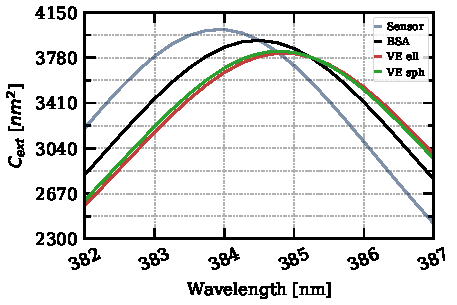
\includegraphics[width=0.85\textwidth]{two_ve_ell_sph_vs_BSA.pdf} 
    \caption{Extinction cross-section as a function of wavelength for an $8$ nm
    silver sphere immersed in water, under a constant electric field, with two volume equivalent 
    ellipsoids/spheres placed $\pm 1$ nm away from the surface in the $z$-direction.}
    \label{fig:sph_vs_ell_ve}
 \end{figure}

We still have the problem of over estimating the shift by $50$ $\%$ compared to the BSA protein original mesh, 
and at first sight we can consider this model comparable to the ellipsoidal volume-equivalent one. However, 
when we use a spherical model for the protein we lose any information regarding the orientation of the protein. 


 \subsubsection{Effect of protein orientation}

 Until this point we always kept the orientation of the proteins such that the dipole moment was parallel to the $y$-axis. In this 
 section we explore the effects of the protein orientation respect to the nanoparticle in the LSPR response. For this study we use the 
 volume equivalent ellipsoids in three different orientations: the original configuration where the dipole moment is parallel to 
 the $y$-axis, a configuration such that the principal axis $a$ is parallel to $y$-axis, 
 and finally a configuration where the principal axis $b$ is parallel to $y$ (see Figure \ref{fig:two_ve_conf_display} for display configurations). Figure \ref{fig:two_ell_mult_config}
 show the LSPR response to the proteins/ellipsoids for the different orientations. 
 
 
 \begin{figure} %[h] %  figure placement: here, top, bottom, or page
    \centering
    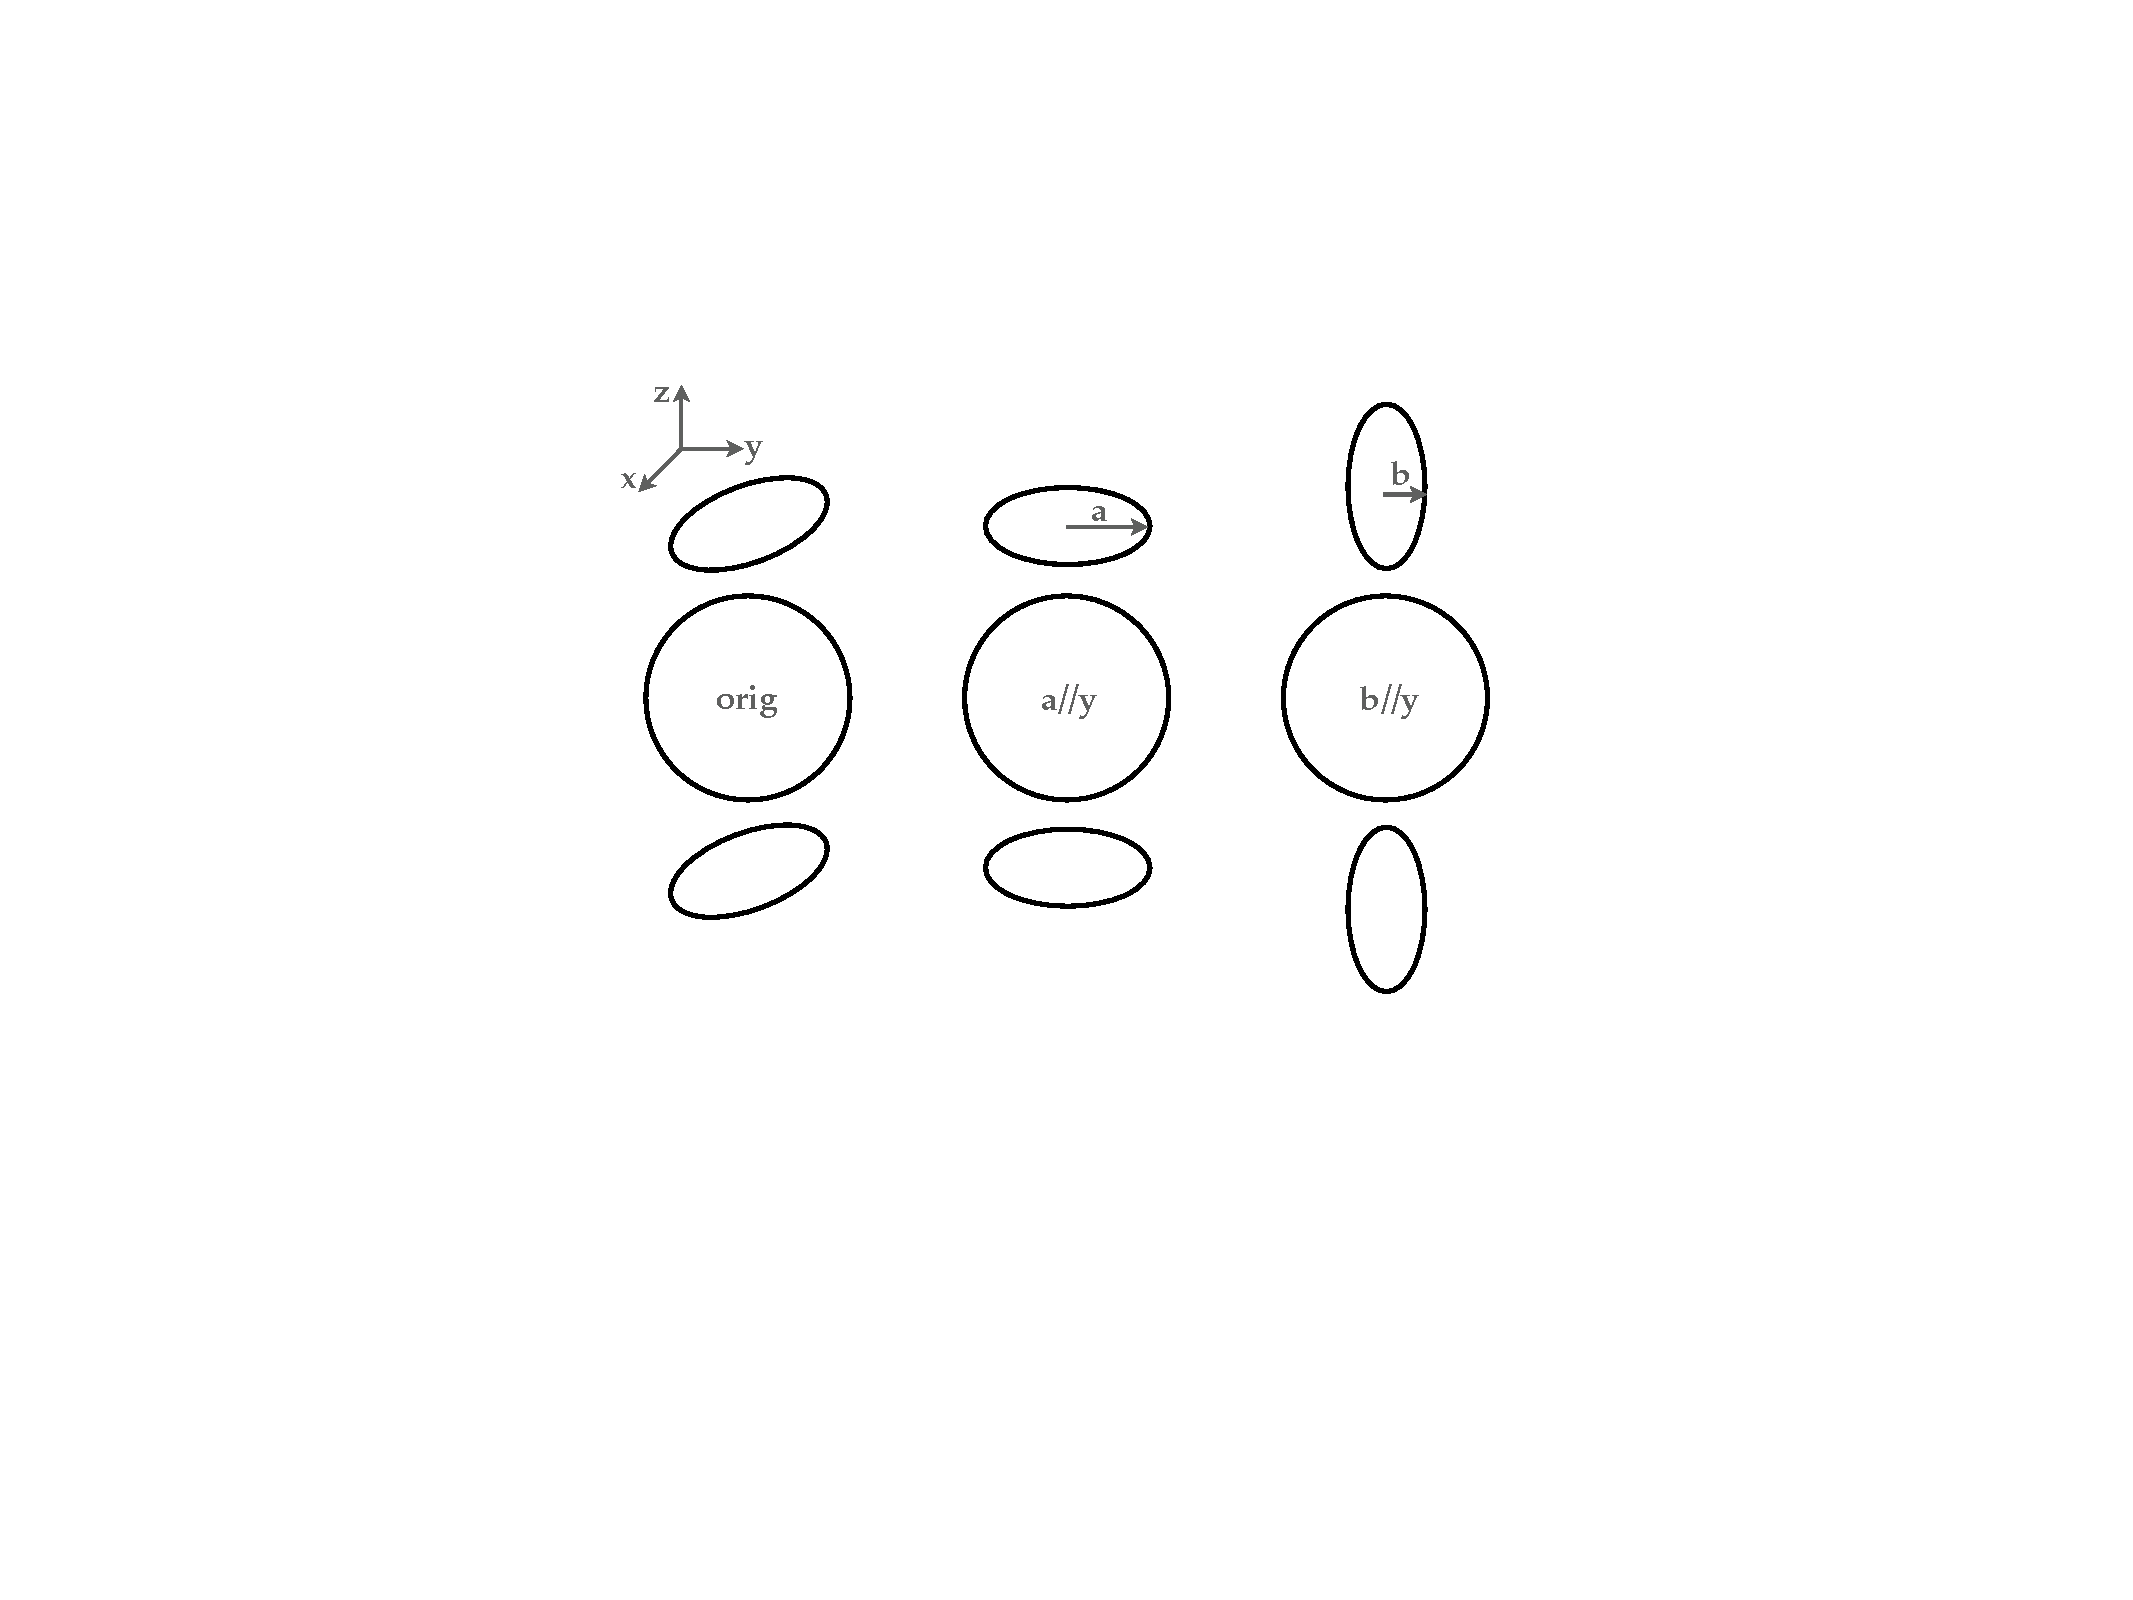
\includegraphics[width=0.65\textwidth]{viz/two_ve_conf_display.pdf} 
    \caption{Different configurations for two volume equivalent ellipsoids.}
    \label{fig:two_ve_conf_display}
 \end{figure}


 
 \begin{figure} %[h] %  figure placement: here, top, bottom, or page
     \centering
     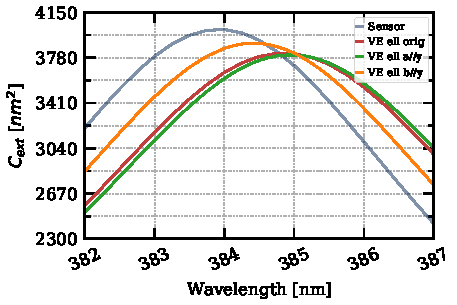
\includegraphics[width=0.85\textwidth]{two_ve_ell_mult_config.pdf} 
     \caption{Extinction cross-section as a function of wavelength for an $8$ nm
     silver sphere immersed in water, under a constant electric field, with two BSA ellipsoids placed 
     $\pm 1$ nm away from the surface in the $z$-direction. "VE ell orig": dipole moment parallel to the $y$-axis,
     "VE ell a//y": principal axis $a$ is parallel to $y$-axis, and "VE ell b//y": principal axis $b$ is parallel to $y$-axis}
     \label{fig:two_ell_mult_config}
  \end{figure}
 


\subsubsection{Effect of number of proteins}

\begin{figure} %[h] %  figure placement: here, top, bottom, or page
    \centering
    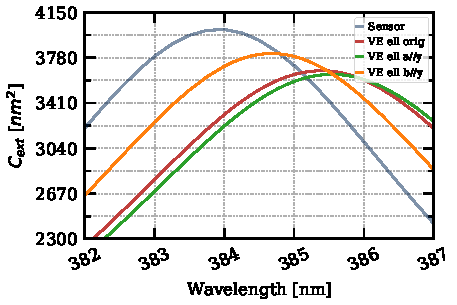
\includegraphics[width=0.85\textwidth]{six_ve_ell_mult_config.pdf} 
    \caption{multiple ell.}
    \label{fig:}
 \end{figure}

\subsubsection{Effect of magnitude of electric field}

\begin{figure}%[t] %  figure placement: here, top, bottom, or page
    \centering
    \subfloat{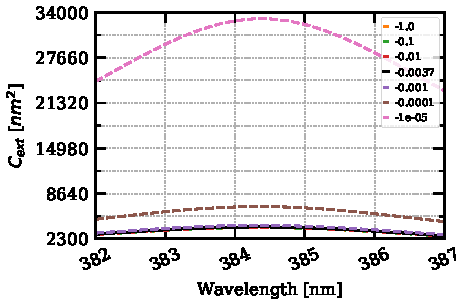
\includegraphics[width=0.85\textwidth]{VE_ell_cm_elec_field_var.pdf}}\\
    \subfloat{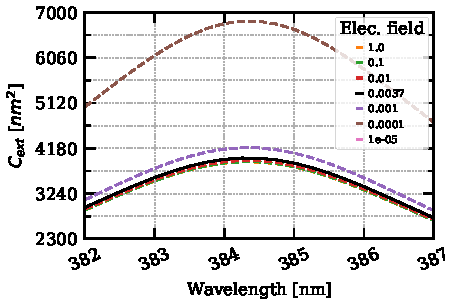
\includegraphics[width=0.85\textwidth]{VE_ell_cm_elec_field_var_zoom.pdf}} 
    \caption{Effect of Electric field, labels are magnitude in [put units here], bottom is zoom}
    \label{fig:efield effect}
 \end{figure}

 \section{Dielectric study}

Most computational works in the literature use a constant real dielectric value both in the protein and the
embedding medium \cite{NghiemETal2012, SantiagoCordobaETal2011,UngerETal2009}, such modeling does not count for the losses 
in that medium. LSPR biosensors detect a target molecule by monitoring plasmon resonance frequency changes due to the proximity 
of the target to the metallic nanoparticle. In this section we show how the LSPR response changes when choosing different models 
for the dielectric in the protein and the medium around the system sensor-protein. We use the same setup used in chapter \ref{hap:lspr_response_bsa}
where we have two BSA proteins located at $\pm$ 1 nm on the $z$-direction of a silver nanoparticle of radius $r=8$ nm (see 
Figure \ref{fig:display_z}). The system sensor-protein is submerged in water and under a constant electric field of 
$0.0037$ $[e]/([{\text{\AA}}^2][\epsilon_0])$ in the $z$-direction. We firstly study the effect of having a real-valued dielectric 
for the protein, by keeping the medium dielectric as complex, secondly we analyze the effect of the medium by using a real-valued 
dielectric for it but keeping the BSA dielectric complex, and finally we study the effect of certain combination where both the medium 
and the protein have real-valued dielectrics. We obtained the values for the real dielectric of the BSA and water (medium) from the literature,
in most cases they provided the refractive index $n$ which we convert to the real dielectric $e_r=n^2$:  

\paragraph{BSA dielectric values:}
\begin{itemize}
    \item {Nghiem et al 2012 \cite{NghiemETal2012}: $n=1.9$, $e_r = n^2 = 3.61$}
    \item {Santiago-Cordoba et al 2011 \cite{SantiagoCordobaETal2011}: $n=1.45$, $e_r = n^2 = 2.0125$}
    \item {Phan et al 2013 \cite{PhanETal2013}: Average of real values of complex Lorentz-Drude model $e_r = 2.7498$}
\end{itemize}

\paragraph{Water dielectric values:}
\begin{itemize}
    \item {Real dielectric of water at room temperature $n=1.33$, $e_r = n^2 = 1.7689$}
    \item {Hale and Querry 1972 \cite{HaleQuerry1972}: Average of experimental real values $e_r = 1.7962$}
\end{itemize}
  
